\documentclass[11pt]{relatorioFisExp}%%% v1.9 de Rui Agostinho, 27/Mar/2018
%%
%% a LISTA EXAUSTIVA de todos os comandos, op??es e packages usadas neste
%% estilo 'relatorioFisExp' est? na file 'helpEstilo_relatorioFisExp.pdf'
%%
%% ----------------------------------
%% A 1? linha ? OBRIGAT?RIA e indica qual ? o estilo de formata??o a usar,
%% que est? na file "relatorioFisExp.cls", a qual deve estar na mesma pasta.
%%
%%>> DEVE usar a op??o 'utf8' se for esta a codifica??o usada nos caracteres 
%%   das files de texto: o seu 'relat?rio.tex' e na 'relatorioFisExp.cls'   
%%          \documentclass[11pt,utf8]{relatorioFisExp}
%%
%% A op??o 11pt define o tamanho base da letra. Pode escolher 10pt ou 12pt,
%%  mas sugere-se que use os 11pt.
%%
%% HELP  estou em p?nico com estas op??es!!!
%%       Para ver a lista de todos os comandos e opcoes dispon?veis
%%                     acrescente a op??o 'help'
%%  ex:   \documentclass[11pt,help]{relatorioFisExp}
%%
%% Para ter um ?ndice no in?cio (antes do Resumo) acrescente a op??o 'indice'
%%  ex:   \documentclass[11pt,indice]{relatorioFisExp}
%%
%% Para ter a folha de rosto com aspecto de artigo, em vez do bloco em formato
%%  de relat?rio que identifica a Turma, Grupo, Aula, etc., use a op??o 'paper'
%%   ex:   \documentclass[11pt,paper]{relatorioFisExp}
%%
%%  Pode ver uma descri??o sucinta de todas as 'op??es' dispon?veis neste
%%  estilo usando a op??o:   \documentclass[11pt,helpOpcoes]{relato...}
%%
%%  ----------------------------------
%% COMO COMPILAR O LATEX: 
%% Esta file ? apenas texto simples, que n?o est? formatada convenientemente. 
%% Para criar a file PDF com o seu relat?rio bem formatado deve
%% compilar esta file com o comando  'pdflatex'  2 vezes consecutivas.
%%
%% -----------------------------------------------------------------
%% ---- BREVES NOTAS SOBRE ALGUNS COMANDOS PR?PRIOS DESTE ESTILO ---
%%
%%  Este relat?rio exemplo est? repleto de exemplos destes comandos.
%%
%%  Mas a LISTA EXAUSTIVA de todos os comandos, est? na file:
%%      'helpEstilo_relatorioFisExp.pdf'   VEJA-A.
%%
%%  acabada esta fofoca....
%%
%%%%%%%%%%%%%%%%%%%%%%%%%%%%%%%%%%%%%%%%%%%%%%%%%%%%%%%%%%%%%%%%%%%%%%%%%%
%%%%%  PRE?MBULO DO DOCUMENTO - DEFINI??ES DE COMANDOS OBRIGAT?RIOS %%%%%%
%%%%%%%%%%%%%%%%%%%%%%%%%%%%%%%%%%%%%%%%%%%%%%%%%%%%%%%%%%%%%%%%%%%%%%%%%%
%% Se quiser alterar o nome da U.Curricular altere pondo
%%           [nome abreviado]{Nome completo}
\NomeDoCurso[Fis.\ Exp.\ I]{F�sica Experimental I}%%% 
%%   --> o predefinido ? 'F?sica Experimental I' => pode apagar esta linha
%%
%% Se quiser alterar o nome da Institui??o (departamento, centro de 
%%  de investiga?ao, etc.) altere-o com
%%          {Nome completo que pretende}
\Instituicao{Departamento de F?sica}%%%  opcional
%%-> predefinido= 'Departamento de F?sica' => pode apagar esta linha

%%%%%%%%        [nome abreviado]{nome completo do trabalho Laboratorial}
\nomeDoTrabalho[Energia Mec?nica]{A Conserva��o da Energia Mec�nica}

%%%% pessoas do grupo que fez o trabalho laboratorial
%%%% [n.aluno]{Nome da Pessoa}
\autorA[12345]{Susana Marta}%% \autorA tem de existir!
\autorB[23456]{Ant?nio Maria}%%% se vazio {} retira o nome do relat?rio
\autorC[34567]{Joaquina R. Migueis}%%% se vazio {} retira o nome do relat?rio
\autorD[45678]{Manuel K.\ Jos?}%%% se vazio {} retira o nome do relat?rio
%%
%% SE usou 'paper' nas op??es (=>formato +artigo) ent?o pode usar:
%% \autorA[email@aqui.pt]{Nome da Pessoa}
%% O email (ou outro texto que aqui use) aparece em rodap? na 1? p?gina.

\dataDoRelatorio{27 de Mar?o}%%% apenas dia e m?s

\ano{2018}%%% o ano em que se realiza a cadeira (UC).

%%% dados da Aula Laboratorial:
\Turma{PL-23}%% designa??o da turma. Ex: PL-22

\GrupoNum{1}%%% n?mero do grupo a que pertencem os autores

\dataAulaLaboratorial{26 de Fevereiro}%%% apenas dia e m?s

\NomeDocenteLab{Rui J.\ Agostinho}%% 



%% se tiver as imagens noutras pastas, acrescente aqui o respetivo  
%% 'pathAbsoluto' e descomente (ao in?cio) a linha seguinte
%\graphicspath{{path1/}{path2/}}%%  os 'path' devem terminar em '/'

%%%%%%%%%%%%%%%%%%%%%%%%%%%%%%%%%%%%%%%%%%%%%%%%%%%%%%%%%%%%%%%%%%%%%
\begin{document}%%% inicia a estrutura de texto do relat?rio
%%%%%%%%%%%%%%%%%%%%%%%%%%%%%%%%%%%%%%%%%%%%%%%%%%%%%%%%%%%%%%%%%%%%%
%%%%%%%%%%%%%%%%%%%%%%%%%%%%%%%%%%%%%%%%%%%%%%%%%%%%%%%%%%%%%%%%%%%%%
%% apresente um BREVE RESUMO do trabalho: 
%%  - objectivos cient?ficos, 
%%  - m?todos experimentais usados
%%  - um resumo dos resultados alcan?ados, com 
%%  - avalia??o cr?tica dos mesmos.

\begin{abstract} %% in?cio do resumo
Estudou-se o valor da acelera??o grav?tica \textit{g} no laborat?rio C1.4.31 da FCUL.
Para tal utilizou-se a queda livre de uma pessoa. Ap?s fazerem-se alguns lan?amentos, 950 vezes no total, para al?m de deduzir que $g_{C1}= 9,801 \pm 0,004\, m/s^2$, demonstra-se que cair n?o faz bem ? sa?de. Dos dados obtidos tamb?m se deduz, com um intervalo de confian?a de 99,5\%, que a gravidade dos hematomas ? proporcional ? altura da queda, ou seja, ? energia cin?tica de embate: $E_c=\frac{1}{2}m v^2$. Por isso, devido ? conserva??o da energia total, conclui-se que ? melhor cair na Lua onde $g_L\approx g_\oplus/6$.
\end{abstract} %% fim do resumo
%% NOTA: o modo matem?tico $mathCode$ apresenta a equa??o descrita por 
%%  'mathCode' em linha com o texto.



%%%%%%%%%%%%%%%%%%%%%%%%%%%%%%%%%%%%%%%%%%%%%%%%%%%%%%%%%%%%%%%%%%%%%
%%%% DEVE APAGAR os textos das NOTAS Explicativas  no seu relat?rio
%%%%%%%%%%%%%%%%%%%%%%%%%%%%%%%%%%%%%%%%%%%%%%%%%%%%%%%%%%%%%%%%%%%%%
\vspace*{-5mm} %%% vertical space -5mm: puxa o par?grafo 5mm para cima
\notasExplicativasEstruturaRelatorio%%% eliminar esta linha
\notasExplicativasLaTeX%%% eliminar esta linha


%%%%%%%%%%%%%%%%%%%%%%%%%%%%%%%%%%%%%%%%%%%%%%%%%%%%%%%%%%%%%%%%%%%%%
%%%%%%%%%%%%%%%%%%%%%%%%%%%%%%%%%%%%%%%%%%%%%%%%%%%%%%%%%%%%%%%%%%%%%
\section{Objetivos do Trabalho e Aspetos Te?ricos}
%%%%%%%%%%%%%%%%%%%%%%%%%%%%%%%%%%%%%%%%%%%%%%%%%%%%%%%%%%%%%%%%%%%%%

\notasExplicativasObjectivosTrabalho\ %%% eliminar esta linha
\textit{Exemplos}:%%% eliminar esta linha

Estudar a import?ncia do momento de in?rcia na velocidade de rota??o de um corpo, em torno de um eixo pr?prio: a sua depend?ncia na distribui??o de massa em torno do centro de rota??o, assim como a depend?ncia na posi??o de J?piter no c?u ? 5$^a$ feira.
%%% A mudan?a de par?grafo (CR) faz-se com uma linha em branco entre eles.
%%% V?rias linhas em branco <==> 1 ?nico CR.
%%% Tamb?m pode ser feito com \par e deixar juntos os dois par?grafos.
%%% Ex: 5$^a$ feira.\par  =>  mudar de par?grafo (CR).
%%% Se usar os dois ao mesmo tempo: \par+linhaEmBranco <==> dois CR.

O objetivo principal ? provar que o disco de Pohl tem uma velocidade de rota??o \textcolor{Blue}{\textbf{\textit{dependente da cor}}} em que est? pintado. Para isso ? necess?rio estudar o seu comportamento com a capacidade de vis?o $V(p)$ dos intervenientes:  
$V(p) =\int_0^\infty\int_0^{2\pi}\hbar \sin(k_B\overline{T}_p(r,\phi))e^{-\alpha.r}\,d\phi\,dr$, 
onde $\overline{T}_p$ ? a temperatura m?dia duma pessoa em queda livre ? dist?ncia $r$ de Plut?o, e as constantes $\hbar$ e $k_B$ s?o as habituais.

%%%%%%%%%%%%%%%%%%%%%%%%%%%%%%%%%%%%%%%%%%%%%%%%%%%%%%%%%%%%%%%%%%%%%
\notasExplicativasAspectosTeoricos\ %% eliminar esta linha
\textit{Exemplos poss?veis:}%%% eliminar esta linha


\subsection{A desacelera??o da rota??o da barra por fric??o aerodin?mica}

Por ser um problema complexo, ? necess?rio considerar as for?as do atrito de fric??o mec?nica $F_f$ e do atrito (arrasto) aerodin?mico $F_{ar}$ que ? proporcional ? velocidade linear $v(r)$ do ponto na barra ? dist?ncia $r$ do centro, assim como a forma geom?trica da barra. 
Calcula-se pelas equa??es do movimento que a velocidade e a acelera??o angulares do sistema variam da seguinte forma:

%%% USO da package 'subfig' que faz floats=figuras ou tabelas lado a lado.
\begin{figure}[H]%% este ? o ambiente de figura
%%% h= here, coloca a fig 'aqui no texto', se couber no resto da p?gina
%%% Se n?o couber a fig ? colocada automaticamente no topo [t]=top 
%%% ou no fim [b]=bottom da p?gina. 
%%% A op??o [!] <=> tenta for?ar a inclus?o neste s?tio
%%% Pode usar combina??es das suas prefer?ncias. Ex: [hbt]
%%% --> A op??o [H] for?a a fig a n?o sair da Sec??o em que est? <--
%%%  Escolha a op??o que reproduza o que pretende ver no texto formatado.
\centering%% conjunto de figs fica centrado na p?gina.
\subfloat[%Caption da subfigure 1:
Velocidade angular da barra $\omega\ (rad/s)$, em fun??o do tempo. Enquanto a massa $m$ cai o $\omega$ aumenta.]%% fim da Caption da subfigure 1
%%%%  1? figura com pouca largura para caberem duas na mesma linha
{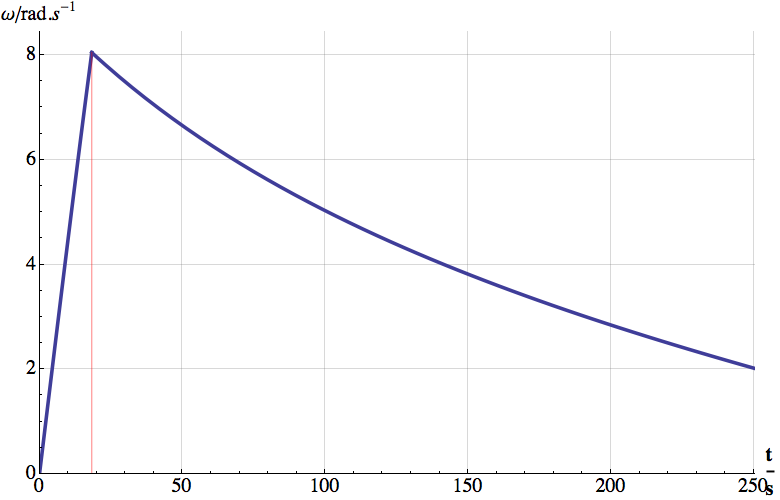
\includegraphics[width=78mm]{velAngMomentoInercia.png}%
 \label{fig:velBarra}
}%% etiquetas a come?ar por 'fig:' referenciam figuras
\qquad%%espa?o horizontal entre as duas figuras
\subfloat%seguido da Caption da subfigure 2:
[Acelera??o angular da barra $\alpha\ (rad/s^2)$, em fun??o do tempo. Sem a massa $m$ a acelera??o $\alpha$ fica negativa.]%% fim da Caption da subfigure 2
%%%%  2? figura com pouca largura para caberem duas na mesma linha
{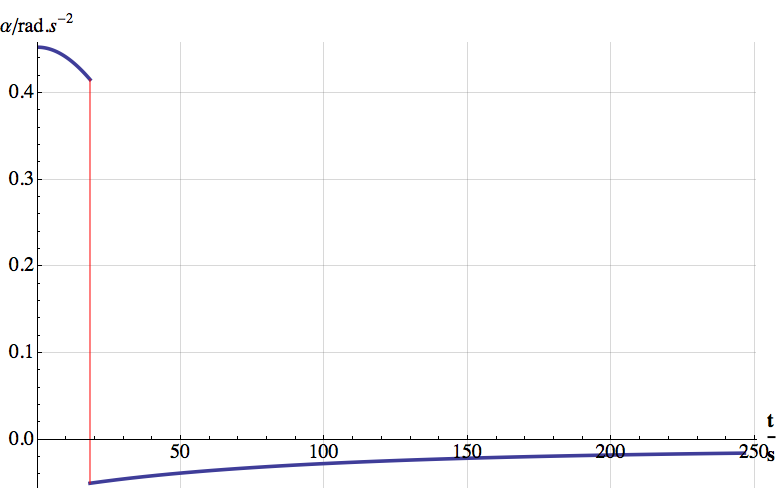
\includegraphics[width=78mm]{acelAngMomentoInercia.png}%
 \label{fig:acelBarra}
}%% 'fig:xx' diferencia as figs dos nomes das equacoes: 'eq:xx'
\caption{%%% legenda comum a todas as sub-figuras
Na parte positiva a acelera??o da massa em queda ? superior ? do atrito, e depois sobra apenas a acelera??o dos atritos de fric??o e aerodin?mico (negativos). S?o valores calculados para as massas cil?ndricas no extremo da barra.}%fim legenda
\label{fig:MomIner}%% etiqueta do conjunto de toda a figura.
\end{figure}
%% O n?mero desta fig. pode ser referenciado por: \ref{fig:MomIner}
%% a p?gina onde a fig. est? ? referenciada por:  \pageref{fig:MomIner}
%% As subfiguras podem ser referenciadas com \subref{fig:velBarra} 
%% e o n?mero da sua p?gina por \pageref{fig:acelBarra}}.


A acelera??o angular $\alpha(t)\!=\frac{d\,\omega(t)}{d\,t}$ a que o sistema fica sujeito n?o ? uniforme e varia conforme apresentado na \referir{fig:acelBarra}. A curvatura vari?vel no comportamento dos dois par?metros $\omega(t)$ (velocidade angular) e $\alpha(t)$, prov?m da for?a de fric??o aerodin?mica $F_{ar}$ que aumenta com a velocidade linear (e a sec??o reta) de embate no ar, $F_{ar}\!\propto v^2$, que aumenta ao longo da barra pois $v\eq\omega\ r$, com $\omega=const$.
%, da densidade m?ssica do ar $\rho_{ar}$ e da sec??o reta de embate no ar.

O extremo da barra sofre maior desacelera??o que a zona central. O bin?rio desta for?a, aplicada na posi??o $r$ ao longo da barra, ? 
$d\overrightarrow{M_{arb}}(r)=\overrightarrow{r}\times C_{ar}\,\rho_{ar}\,dA_b \,v^2\overrightarrow{u_v}$, 
em que $dA_b=D_b\,dr$ ? a ?rea de embate no ar dessa sec??o, $D_b$ o di?metro da espessura da barra e $\rho_{ar}$ a densidade m?ssica do ar. $C_{ar}\approx 0,5$ ? o coeficiente de atrito aerodin?mico que depende da forma do objeto, um cilindro finito neste caso.
A perda de momento angular na rota??o da barra de semi-comprimento $l_b$ ? proporcional ao integral: 
$\,\int_0^{l_b} d\overrightarrow{M}(r)=
I_{tot}\frac{d\,\overrightarrow{\omega}}{d\,t}=
I_{tot}\cdot\overrightarrow{\alpha_b}$, em que $\overrightarrow{\alpha_b}$ ? a acelera??o angular do sistema devida ? travagem aerodin?mica na barra.
O integral resulta em $M_{arb}=\frac{1}{2} C_{ar}\,\rho_{ar}\,D_b\,l_b\,\omega^2$, para a barra completa.

Considerando que existe uma massa cil?ndrica grande $M$ de di?metro $D_M$, comprimento $l_M$ (que tapa a barra), com a 1\upa\ face ? dist?ncia $x_M$ do centro, o integral anterior na barra completa, d?
\begin{subequations}%% comente a linha => numeracao diferente nas equacoes 
\begin{align}
   M_{arb} &= \frac{1}{2}\,C_{ar}\,\rho_{ar}\,D_b \left( l_b^4-(x_M+l_M)^4
     +x_M^4 \right)\omega^2 = K_{arb}\times\omega^2. \\     
   M_{arM} &= \frac{1}{2}\, C_{ar}\,\rho_{ar}\,D_M \left( (x_M+l_M)^4-x_M^4 
     \right)\omega^2 = K_{arM}\times\omega^2 \label{eq:MarM}
\end{align}
\label{eq:MarTot}
\end{subequations}%% comente a linha => numeracao diferente nas equacoes 
\noindent %%% comando que retira a indenta??o na 1? linha do par?grafo
sendo a equa??o \ref{eq:MarM} o bin?rio da for?a aerodin?mica aplicada nas duas massas $M$.

Nos casos estudados e com as massas M perto do centro, $x_M=10,2$ cm, obt?m-se 
$K_{arM}=18,3\,\rm g.cm^2$ e $K_{arb}=144,5\,\rm g.cm^2$: a barra ? dominante. 
A situa??o inverte-se para $x_M=28,2$ cm:  
$K_{arM}=379,5\,\rm g.cm^2$ e $K_{arb}=93,8\,\rm g.cm^2\Rightarrow$ o bin?rio da for?a aerodin?mica aplicada nas duas massas $M$ ? dominante.
%% o modo matem?tico $mathCode$ apresenta a eq. em linha do texto.

\subsubsection{Equa??es do movimento e a determina??o experimental do Momento de In?rcia Total}

A integra??o da equa??o diferencial do movimento tem duas solu??es diferentes: enquanto cai o prato com a massa $m\Rightarrow$ acelera??o inicial, a velocidade $\omega_1(t)$ aumenta; ap?s o instante $t_q$ em que a massa $m$ se desprende o atrito faz a velocidade $\omega_2(t)$ diminuir at? zero. Nas equa??es $I_{tot}$ ? o momento de in?rcia total do sistema, $K_{ar}=K_{arb}+K_{arM}$. No instante $t_q$ a velocidade angular ? $\omega_1(t_q)\eq \omega_2(t_q)\eq \omega_q$. O atrito aerodin?mico (eqs.\ \ref{eq:MarTot}) imp?e uma velocidade limite $\omega_{1max}$ quando $t\!\rightarrow\!\infty$.
\begin{subequations}%% comente a linha => numeracao diferente nas equacoes 
\begin{align}
\text{Sendo\quad} \omega_{1max} &= \sqrt{\frac{r (m g-F_{at})}{K_{ar}}}\text{\quad ent?o,}\\
\omega_1(t) &= \omega_{1max}\tanh \left(\frac{K_{ar}}{I_{tot}+m r^2}\,\omega_{1max}\,t\right) \\
\text{Considerando\quad} W_2 &= \sqrt{\frac{r\,F_{at}}{K_{ar}}}\text{\quad ent?o}\\
\omega_2(t) &= - W_2\tan \left(\frac{K_{ar}}{I_{tot}}\,W_2\,(t-t_q) - \tan^{-1}\left(\frac{\omega_q}{W_2} \right)\right)
\end{align}
\label{eq:omegaIn}
\end{subequations}%% 

\vspace*{-4mm}%
\begin{subequations}%% comente a linha => numeracao diferente nas equacoes 
\begin{align}
\alpha_{1max} &= \sqrt{\frac{r (m g-F_{at})}{I_{tot}+m r^2}}\text{\quad ent?o,}\\
\alpha_1(t) &= \alpha_{1max}\,\text{sech}^2 \left(\omega_{1max} \frac{K_{ar}}{I_{tot}+m r^2}\,t\right) \\
\text{Como\quad} \alpha_{at} &= \frac{r\,F_{at}}{I_{tot}},\\
\alpha_2(t) &= - \alpha_{at}\sec^2 \left(\frac{K_{ar}}{I_{tot}}\,W_2\,(t-t_q) - \tan^{-1}\left(\frac{\omega_q}{W_2} \right)\right)
\end{align}
\label{eq:alfaIn}
\end{subequations}%% 

\vspace*{-8mm}%-8mm
A acelera??o come?a com o valor m?ximo $\alpha_{1max}$ e depois $\alpha_1(t)$ diminui. Ap?s $t_q$ ($m$ desprende-se) passa a $\alpha_{2}(t)\!<\!0$. A acelera??o $\alpha_{at}$ ? devida ? for?a de atrito $F_{at}$ no eixo de raio $r$ e $\alpha_{at}=\alpha_2(t\!\rightarrow\!\infty)$.


O melhor procedimento para determinar o momento de in?rcia total $I_{tot}$ por via da medi??o da rota??o, ? o seguinte: nas curvas $\omega_1(t)$ e $\omega_2(t)$ \textsl{escolha-se um valor qualquer de refer?ncia} $\omega_{ref}$. Nos instantes $t_1$ e $t_2$ que correspondem a 
$\omega_1(t_1) = \omega_2(t_2)=\omega_{ref}$, calcule-se (numericamente a partir dos dados) o valor das acelera??es angulares $\alpha_1(t_1)$ e $\alpha_2(t_2)$. Demonstra-se pelas equa??es \ref{eq:omegaIn} e \ref{eq:alfaIn} que o momento de in?rcia total do sistema ? sempre (exatamente) dado por:

\fequ{
I_{tot}=m\,r\frac{g-r\, \alpha_1(t_1)}{\alpha_1(t_1)-\alpha_2(t_2)}
}

%\vspace*{6mm}
\subsection{Aspetos da oscila??o harm?nica amortecida com um termo de atrito constante}

Integrando a \referir{eq:ajusteVelPohl} obt?m-se a posi??o angular $\theta(t)$ do disco no instante $t$:\quad ($W=\frac{2\pi}{T}$) 
%% As etiquetas das equa??es devem come?ar por 'eq:'
%% etiqueta desta equa??o: eq:teta
%% \fequ[lbl]{mathCodeHere} cria uma equa??o numerada com caixa ? volta
\fequ[eq:teta]{\theta(t)\approx\left(\frac{v_{0}\, e^{\lambda\,t}}{\sqrt{W^2+\lambda^2}}+\frac{a_f}{W^2} \sqrt{1+(t\,W)^2}\right) \sin(t\,W-\frac{\pi}{2})
}
\begin{figure}[H]%%%  h=here => coloque a figura aqui no texto
\centering
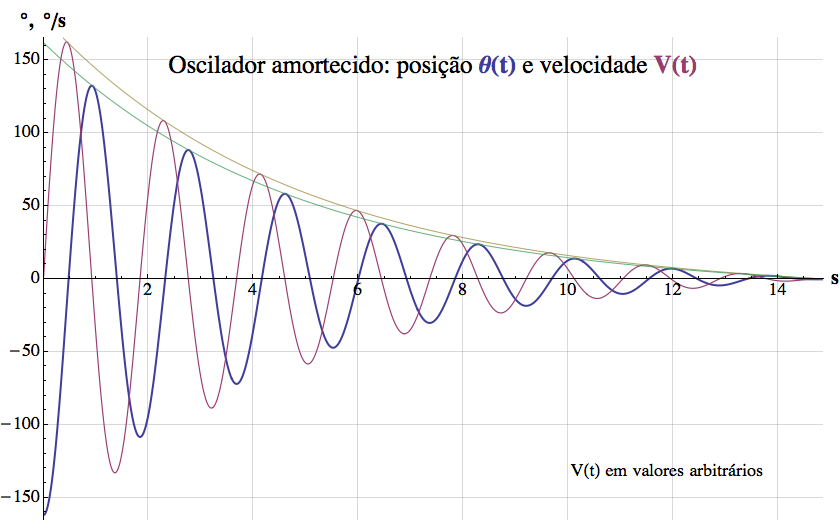
\includegraphics[width=140mm]{OHteoricoA19i400mA.png}
%%% legenda da figura
\caption{Posi??o angular $\theta(t)$ e velocidade linear $V(t)$ de rota??o do disco de Pohl, para as condi??es de i=0,40A e amplitude inicial 19. Nota: a velocidade est? com valores reduzidos para ficar na mesma escala.}
\label{fig:posVelDiscoPohl}%%% etiqueta identificadora desta figura
\end{figure}


Para determinar a constante de amortecimento $\lambda$ deve medir-se o tempo $t_f$ que o oscilador demora a parar: introduzindo na \referir{eq:teta} $\theta(t_f)=0$ e considerando que $W\gg\lambda$, deduz-se uma rela??o que permite estimar $\lambda$: 

%% o modo $$ mathCodeAqui $$ = \[ mathCodeAqui \] apresenta a equa??o num 
%% par?grafo separado SEM numera??o da equa??o
$$
\lambda= \frac{1}{t_f} \ln\left(-\frac{a_f}{v_{0}} \frac{\sqrt{W^2+\lambda^2}}{W^2} \sqrt{1+(t_f W)^2}\right)  \Rightarrow 
\lambda\approx \frac{1}{t_f} \ln\left(\frac{-a_f}{v_{0}W} \sqrt{1+(t_f W)^2}\right) 
$$
A sua utiliza??o depende do conhecimento ? priori do valor da desacelera??o por fric??o $a_f$, caracter?stica de cada disco de Pohl, pois tanto $W$ como $v_0$ s?o  mensur?veis em cada experi?ncia.


%%%%%%%%%%%%%%%%%%%%%%%%%%%%%%%%%%%%%%%%%%%%%%%%%%%%%%%%%%%%%%%%%%%%%
%%%%%%%%%%%%%%%%%%%%%%%%%%%%%%%%%%%%%%%%%%%%%%%%%%%%%%%%%%%%%%%%%%%%%
\section{Procedimentos Experimentais}
%%%%%%%%%%%%%%%%%%%%%%%%%%%%%%%%%%%%%%%%%%%%%%%%%%%%%%%%%%%%%%%%%%%%%

\notasExplicativasProcedimentosExperimentais\ %%% remover esta linha
\textit{Exemplos:}

Para estudar o momento de in?rcia num movimento circular, foi usada uma barra em rota??o, com duas massas maiores $M$ ? mesma dist?ncia do centro de rota??o. O sistema foi colocado em movimento com outra massa $m$ que o puxava enquanto ca?a. Assim, procedeu-se da seguinte maneira:
\begin{itemize}[label=$\surd$]%% produz uma lista n?o numerada
\itemsep -1mm %%% reduz o espa?o vertical entre itens
\item mediu-se o atrito de fric??o do sistema $F_f$,
\item mediu-se o atrito aerodin?mico $F_{aero}$ que ? proporcional ao quadrado da velocidade linear $v(r)$ de um ponto da barra ? dist?ncia $r$ do centro, 
\item mediu-se a forma da barra.
\end{itemize} 


%%%%%%%%%%%%%%%%%%%%%%%%%%%%%%%%%%%%%%%%%%%%%%%%%%%%%%%%%%%%%%%%%%%%%
\subsection{Medi??es e Dados Obtidos}

\notasExplicativasMedicoesDadosObtidos %%% remover esta linha

\subsubsection{Medi??o de oscila??es harm?nicas com o disco de Pohl}

\begin{figure}[H]%%%  h=here => coloque a figura aqui no texto
\centering %% fig centrada na p?gina
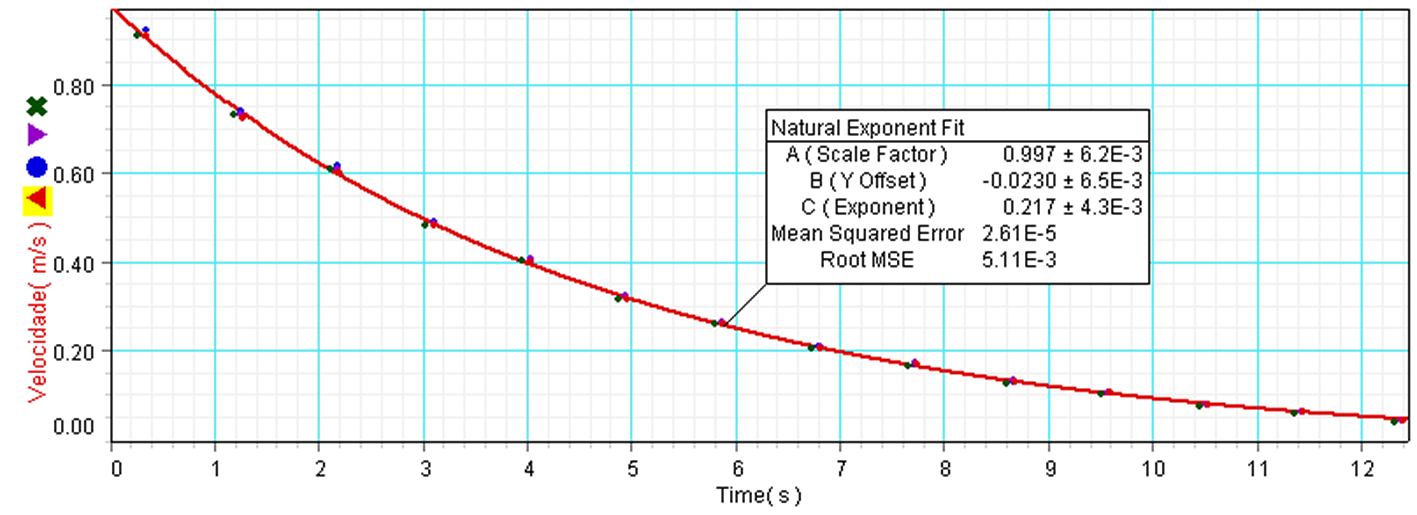
\includegraphics[width=145mm]{HMSvelo_A19i400mA.png}
%%% legenda da figura
\caption{Velocidade linear m?xima de rota??o do disco de Pohl (m/s), em fun??o do tempo.}
\label{fig:velPohldatastudio}%%% etiqueta identificadora desta figura
\end{figure}
  
Lan?ando o disco de Pohl com amortecimento (corrente no eletro?man $i=0,40$ A), ob\-ser\-va-se %% \- indica onde a palavra pode ser hifenada
 a velocidade m?xima a diminuir em cada oscila??o, ou seja, desacelera??o for?ada descrita por uma fun??o exponencial, como se constata na \referir{fig:velPohldatastudio}.% Note que o per?odo n?o permanece constante.

\subsubsection{A Medi??o da Expans?o do Universo}
Os nossos dados s?o os melhores do mundo. Apesar de haverem \textit{ligeiros} problemas nas medi??es, os resultados obtidos s?o t?o bons que ser?o apresentados numa confer?ncia internacional sobre Cosmologia Experimental.
Encontram-se na tabela \ref{tab:dados} os resultados das medi??es efetuadas:

%%Para reduzir o tamanho das tabelas muito grandes usar o \scalebox
%%\scalebox{0.7}{
%%  \begin{tabular}
%%    ...
%%  \end{tabular}
%%}%%fim do scalebox
\begin{table}[h!]%% ambiente de tabela com caption e label
%%% pode ter v?rias tabelas (tabular) l? dentro
\centering %% conjunto de tabelas centrado na p?gina
%%%%  1? tabela com 3 colunas
\begin{tabular}{ccc}%% ccc= as 3 com texto 'c' de 'centrado'
\toprule 
%%  o s?mbolo '&' separa o texto nas colunas:  t1 & t2 & t3 \\
t {\small(s)} & $\omega$ {\small(rad/s)} & $\Omega$\\%% 1?linha=cabe?alho
\midrule  
0,1 & \Exp{17,8}{1} & 0,30\\%% dados da 2?linha
0,4 & \Exp{34,1}{2} & 0,31\\%% dados da 3?linha
0,5 & \Exp{56,2}{2} & 0,29\\%% dados da 4?linha
\bottomrule
\end{tabular}%% termina da 1? tabela de valores
\hspace{15mm}%% espa?o horizontal entre elas, ou \quad ou \qquad
%%%% 2? tabela s? com 3 colunas tamb?m. Para ficar na mesma
%%%% linha da 1? tab, N?O pode haver aqui uma linha em branco
\begin{tabular}{@{}ccc@{}}%% @{} retira espa?o extra nos extremos
\toprule 
%%  as c?lulas nas colunas s?o separados por '&':  1 & 2 & 3 \\
$\hbar$ {\small(J.s)} & $|\overrightarrow{v}|_{max}${\small(m/s)} & 
$a$ {\small(m/s$^2$)}\\%%1? linha=cabe?alho
\midrule 
0,100 & 17,8 & 0,030\\%% dados da 2?linha
0,410 & 34,1 & 0,031\\%% dados da 3?linha
0,578 & 56,2 & 0,029\\%% dados da 4?linha
\bottomrule
\end{tabular}%% termina da 2? tabela de valores
%%% legenda da figura
\caption{Medi??es da rota??o $\omega$ do universo e da sua densidade energ?tica relativa $\Omega$, obtidas com o telesc?pio de 20 metros de di?metro no laborat?rio C1.4.31 da FCUL.}
\label{tab:dados}%%% etiqueta identificadora destas tabelas
%% as etiquetas das tabelas devem come?ar por 'tab:'
\end{table}

\subsubsection{Dados do per?odo e velocidade m?xima do p?ndulo}

Os colegas Eduardo, Andr? e Jo?o mediram o per?odo do pequeno p?ndulo em cima da bancada, a quem se agradece muito partilharem os dados.
%Comprimentos $l=50,0\pm0,05$cm e $l=24,2\pm0,05$cm.

%%%  Para reduzir o tamanho das tabelas, use o comando \scalebox. Ex:
%%%  \scalebox{0.7}{
%%%   \begin{tabular}
%%%    ...
%%%   \end{tabular}
%%%  }
\begin{table}[H]
\centering
\scalebox{0.75}{%% <<-- reduz todo o texto para 75%
\begin{tabular}{c}
\toprule
\textbf{$T_1$  (s)}\\ 
\midrule
1,3447\\  1,3444\\  1,3445\\  1,3447\\  1,3446\\  1,3445\\  1,3445\\
1,3445\\  1,3444\\  1,3445\\  1,3444\\  1,3444\\  1,3445\\  1,3445\\
1,3445\\  1,3444\\  1,3444\\  1,3444\\  1,3444\\  1,3443\\  1,3443\\
1,3444\\  1,3443\\  
%1,3443\\  1,3442\\  1,3442\\  1,3441\\  1,3443\\
%% nao cabem na pagina
% 1,3442\\  1,3441\\  
\bottomrule
\end{tabular}
\hspace{20mm}
%%%%%  esta tabela ? enorme em altura: fiz-lhe duas colunas
\begin{tabular}{cc}%
\toprule
\multicolumn{2}{c}{\textbf{$V_1$ (m/s)}}\\ 
\midrule
0,1523 & 0,1339\\  0,1531 & 0,1351\\  0,1515 & 0,1327\\  0,1515 & 0,1333\\
0,1493 & 0,1316\\  0,1493 & 0,1327\\  0,1478 & 0,1304\\  0,1485 & 0,1316\\ 
0,1463 & 0,1288\\  0,1471 & 0,1304\\  0,1456 & 0,1282\\  0,1463 & 0,1293\\
0,1442 & 0,1271\\  0,1449 & 0,1282\\  0,1429 & 0,1261\\  0,1442 & 0,1271\\
0,1415 & 0,1250\\  0,1422 & 0,1261\\  0,1408 & 0,1240\\  0,1415 & 0,1255\\
0,1395 & 0,1230\\  0,1408 & 0,1240\\  0,1389 & 0,1220\\ 
%% nao cabem na pagina 
% 0,1395 & 0,1230\\  
%0,1370 & 0,1210\\  0,1382 & 0,1224\\  0,1357 & 0,1195\\  0,1370 & 0,1210\\
%0,1351 & 0,1190\\  0,1357 & 0,1176\\  
\bottomrule
\end{tabular}
\hspace*{20mm}
\begin{tabular}{c}
\toprule
\textbf{$T_2$ (s)}\\ 
\midrule
1,1486\\  1,1487\\  1,1484\\  1,1482\\  1,1483\\  1,1480\\  1,1480\\  
1,1479\\  1,1478\\  1,1477\\  1,1474\\  1,1472\\  1,1470\\  1,1465\\  
1,1460\\  1,1453\\  1,1454\\  1,1455\\  1,1447\\  1,1449\\  1,1446\\  
1,1443\\  1,1444\\ 
%% nao cabem na pagina 
% 1,1430\\  1,1433\\  1,1441\\  1,1430\\  1,1435\\  1,1431\\  1,1434\\  
\bottomrule
\end{tabular}
\hspace{16mm}
\begin{tabular}{cc}
\toprule
\multicolumn{2}{c}{\textbf{$V_2$ (m/s)}}\\ 
\midrule
0,2747  &  0,1605\\  0,2740  &  0,1553\\  0,2653  &  0,1543\\  
0,2646  &  0,1493\\  0,2577  &  0,1484\\  0,2577  &  0,1443\\  
0,2494  &  0,1425\\  0,2488  &  0,1385\\  0,2410  &  0,1368\\  
0,2398  &  0,1330\\  0,2331  &  0,1316\\  0,2320  &  0,1277\\
0,2252  &  0,1272\\  0,2232  &  0,1225\\  0,2179  &  0,1221\\  
0,2155  &  0,1176\\  0,2101  &  0,1174\\  0,2083  &  0,1115\\  
0,2024  &  0,1112\\  0,2008  &  0,1059\\  0,1949  &  0,1064\\  
0,1938  &  0,1019\\  0,1876  &  0,1017\\ 
%% nao cabem na pagina
% 0,1869  &  0,0973\\ 0,1805  &  0,0973\\  0,1802  &  0,0940\\ 
%0,1736  &  0,0936\\  0,1733  &  0,0904\\
%0,1675  &  0,0904\\  0,1669  &  0,0866\\ % 0,1616  &  0,0863\\  
\bottomrule
\end{tabular}
}%%% <<-fim do scalebox que reduziu o tamanho da tabela
\caption{Dados obtidos no primeiro ensaio de medi??o do per?odo com o DataStudio. \textbf{Nota:} Os valores de velocidade e per?odo n?o foram obtidos durante o mesmo ensaio. Os da velocidade $V_1$ s?o do ensaio realizado com o comprimento do fio $l=50$ cm e os da $V_2$ s?o para $l=24,2$cm}
\label{tab:dados1.1DataStudio}
\end{table}



\subsubsection{Dados da Conserva??o da Energia Mec?nica}

No laborat?rio utilizou-se uma calha de ar inclinada de um ?ngulo $\alpha$, na qual foram lan?ados um carrinho em deslize (sem rota??o), uma esfera e um cilindro, ambos em rota??o. Foi sempre medida a posi??o inicial (de repouso) na calha em rela??o ? posi??o final, a do fotoporta que media a velocidade e que permaneceu fixo na parte inferior da calha em todos os lan?amentos. A dist?ncia da posi??o inicial foi medida com a fita m?trica que existe ao longo da calha.  Os resultados das experi?ncias foram gentilmente cedidos pelas colegas Elsa, In?s e V?nia, a quem se agradece muito.
\begin{figure}[H]%%%  h=here => coloque a figura 'aqui' no texto
%%%%  a op??o H ? um 'h' mais forte: obriga a coloca??o da fig 'mesmo aqui'
\centering %% fig centrada na p?gina
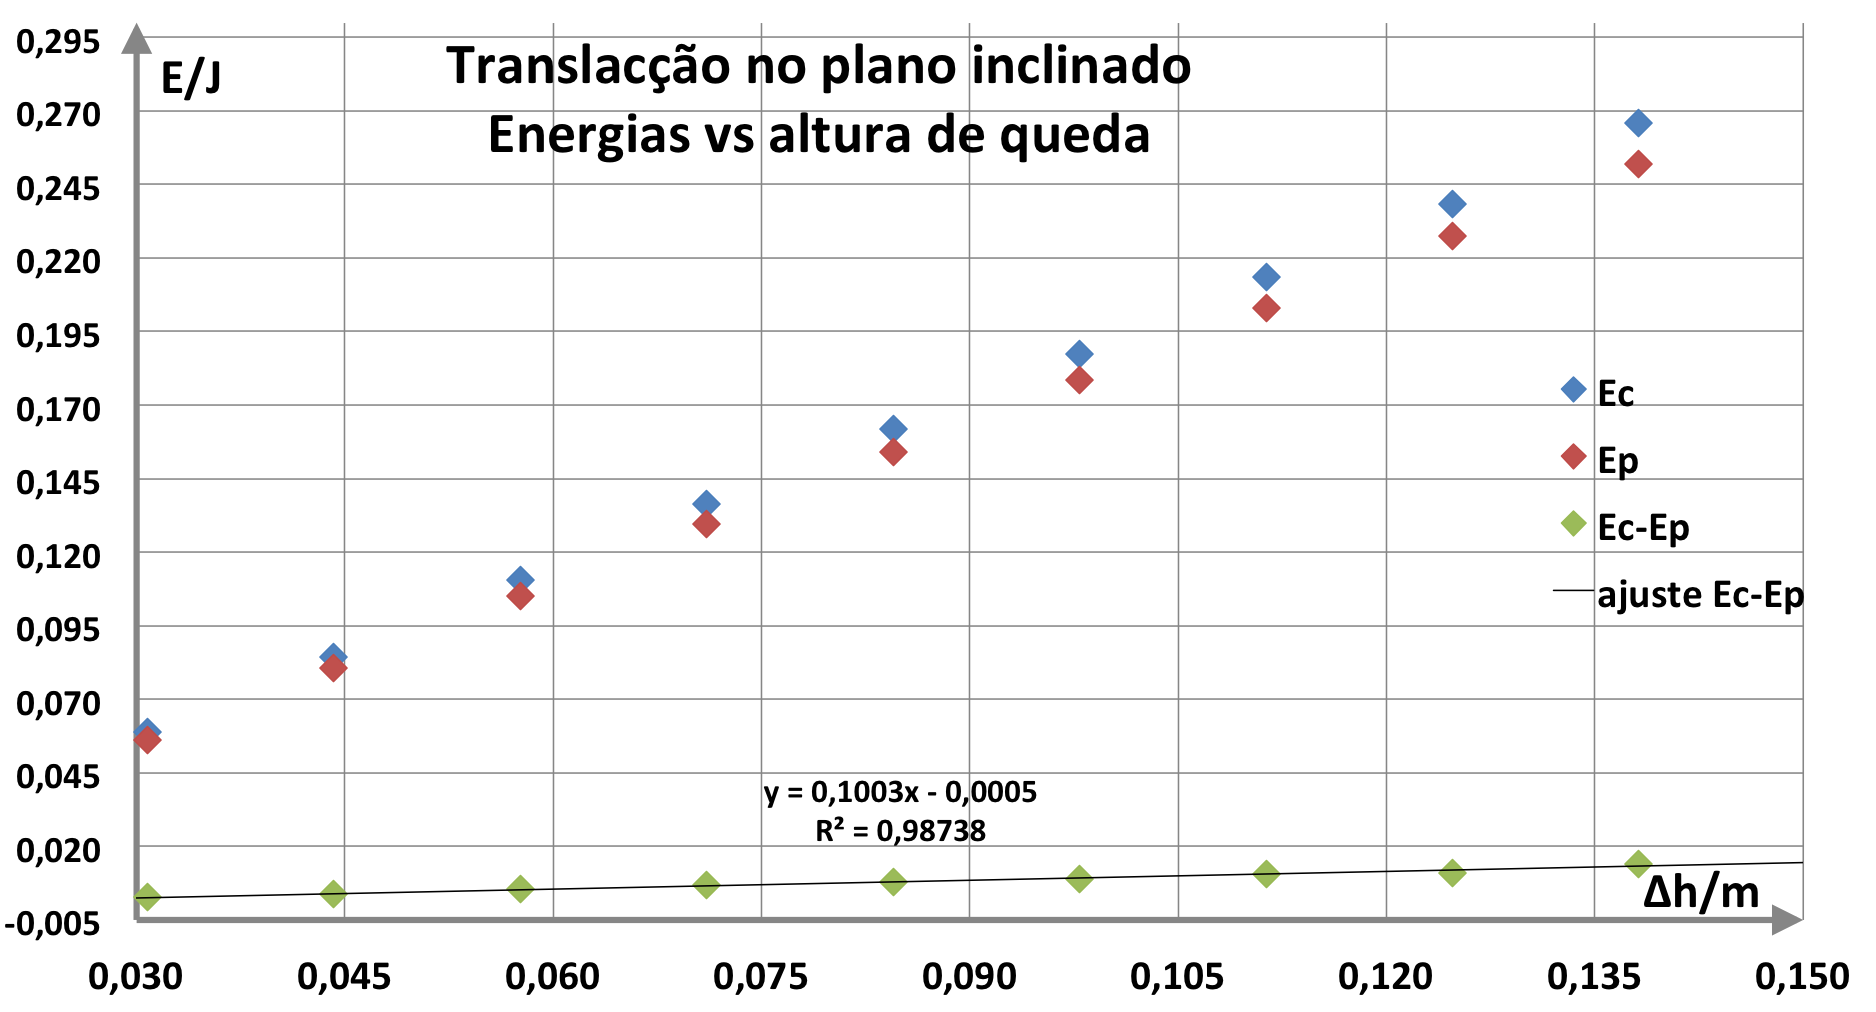
\includegraphics[width=110mm]{translacaoPlanoInclinadOrig.png}
%%% legenda da figura
\caption{Lan?amentos do Carrinho no plano inclinado: energias cin?tica final (Ec), potencial inicial (Ep) e a sua diferen?a (Ec-Ep) em Joules, em fun??o da altura relativa de queda $\Delta h$(m). Par?metros originais.}
\label{fig:carroOri}%%% etiqueta identificadora desta figura
\end{figure}

Para o lan?amento do carrinho os resultados encontram-se no gr?fico \ref{fig:carroOri}: torna-se estranho que exista mais energia cin?tica (? chegada) do que a potencial inicial.

No lan?amento da esfera em transla??o e rota??o os resultados constam na \referir{fig:esferaOri}. Note-se que a medi??o referente aos 2,8 cm de altura deve ter sido mal feita, devido ao desvio inverso ao comportamento dos outros dados. Novamente h? um aumento de energia total do sistema: a cria??o de energia a partir do nada d? um Pr?mio Nobel!
\begin{figure}[h!]
%%%  h=here => coloque a figura 'aqui' no texto
\centering %% fig centrada na p?gina
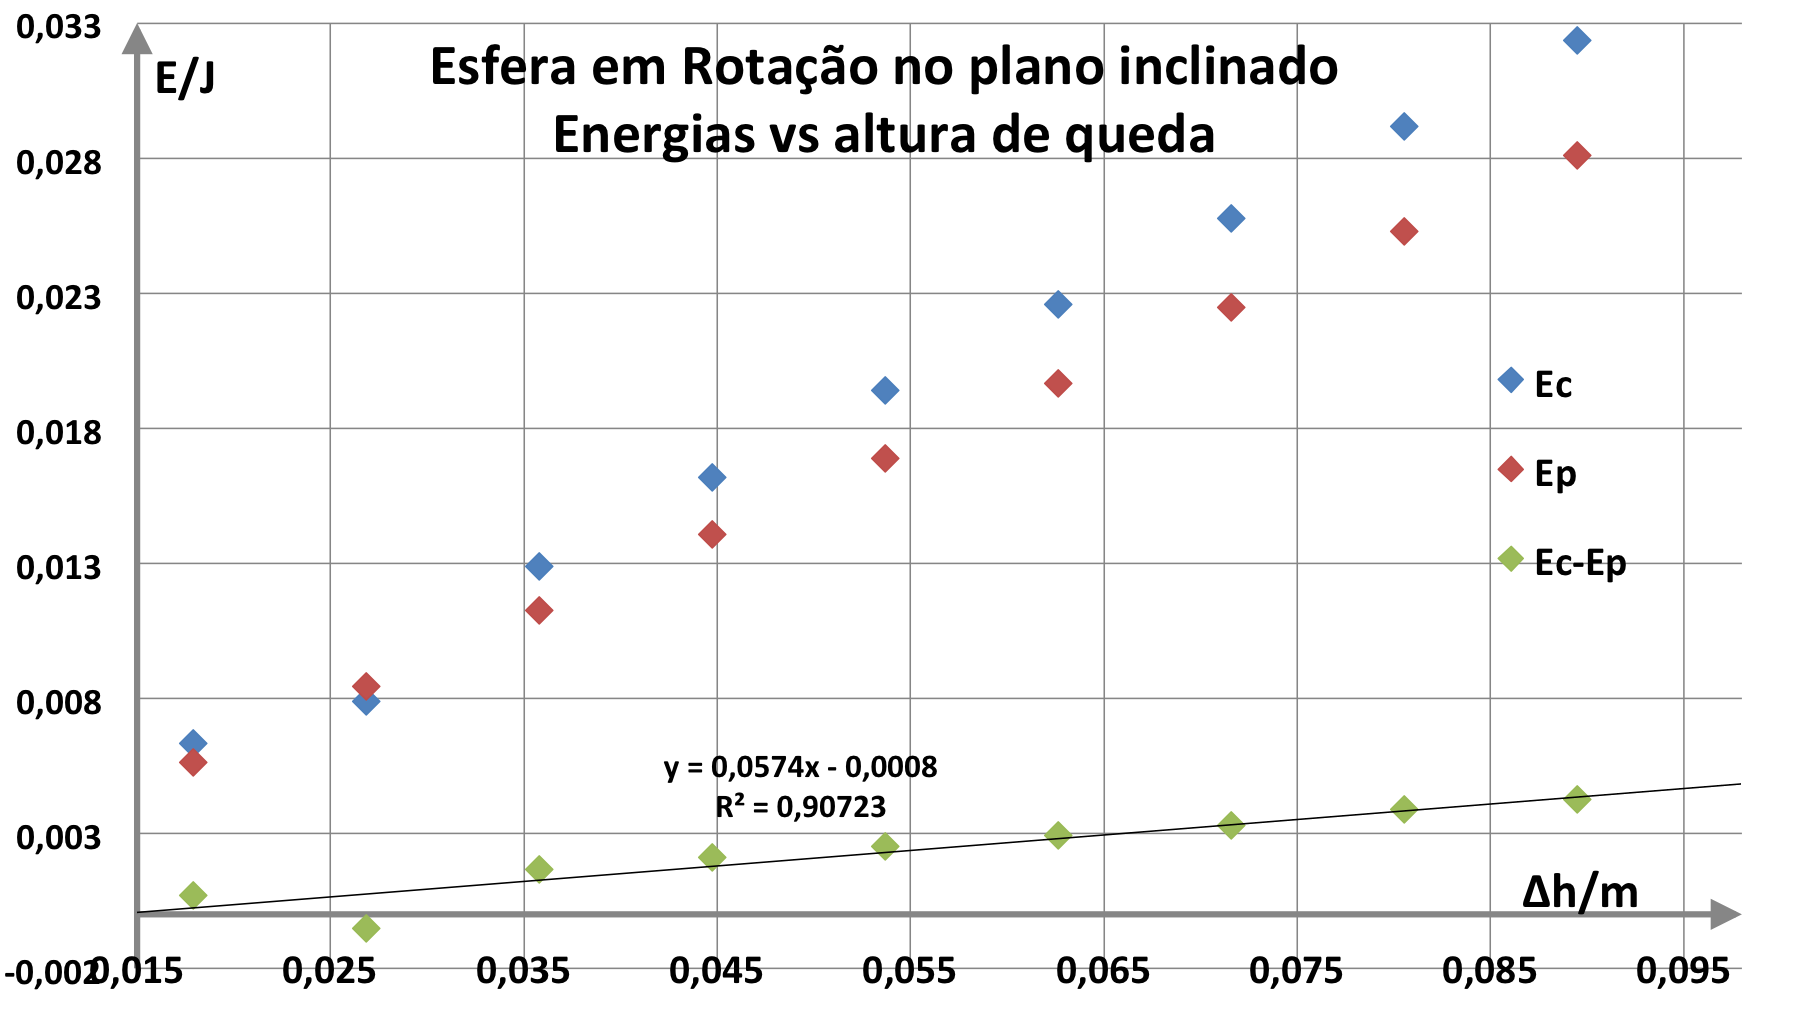
\includegraphics[width=120mm]{esferaPlanoInclinadOrig.png}
%%% legenda da figura
\caption{Esfera com rota??o no plano inclinado: energias cin?tica final (Ec), potencial inicial (Ep) e a sua diferen?a (Ec-Ep) em Joules, em fun??o da altura relativa de queda $\Delta h$(m). Par?metros originais.}
\label{fig:esferaOri}%%% etiqueta identificadora desta figura
\end{figure}

O lan?amento do cilindro a diversas alturas iniciais teve os resultados apresentados na figura \ref{fig:cilindroOri}. Nesta situa??o aparece uma perda de energia total: a energia cin?tica $E_c$ final ? inferior ? energia potencial $E_p$ inicial, o que est? de acordo com o expect?vel: perda de energia total por atrito de rolamento e um pouco de atrito aerodin?mico (pouco, devido ? baixa velocidade).
\begin{figure}[h!]
%%%  h=here => coloque a figura 'aqui' no texto
\centering %% fig centrada na p?gina
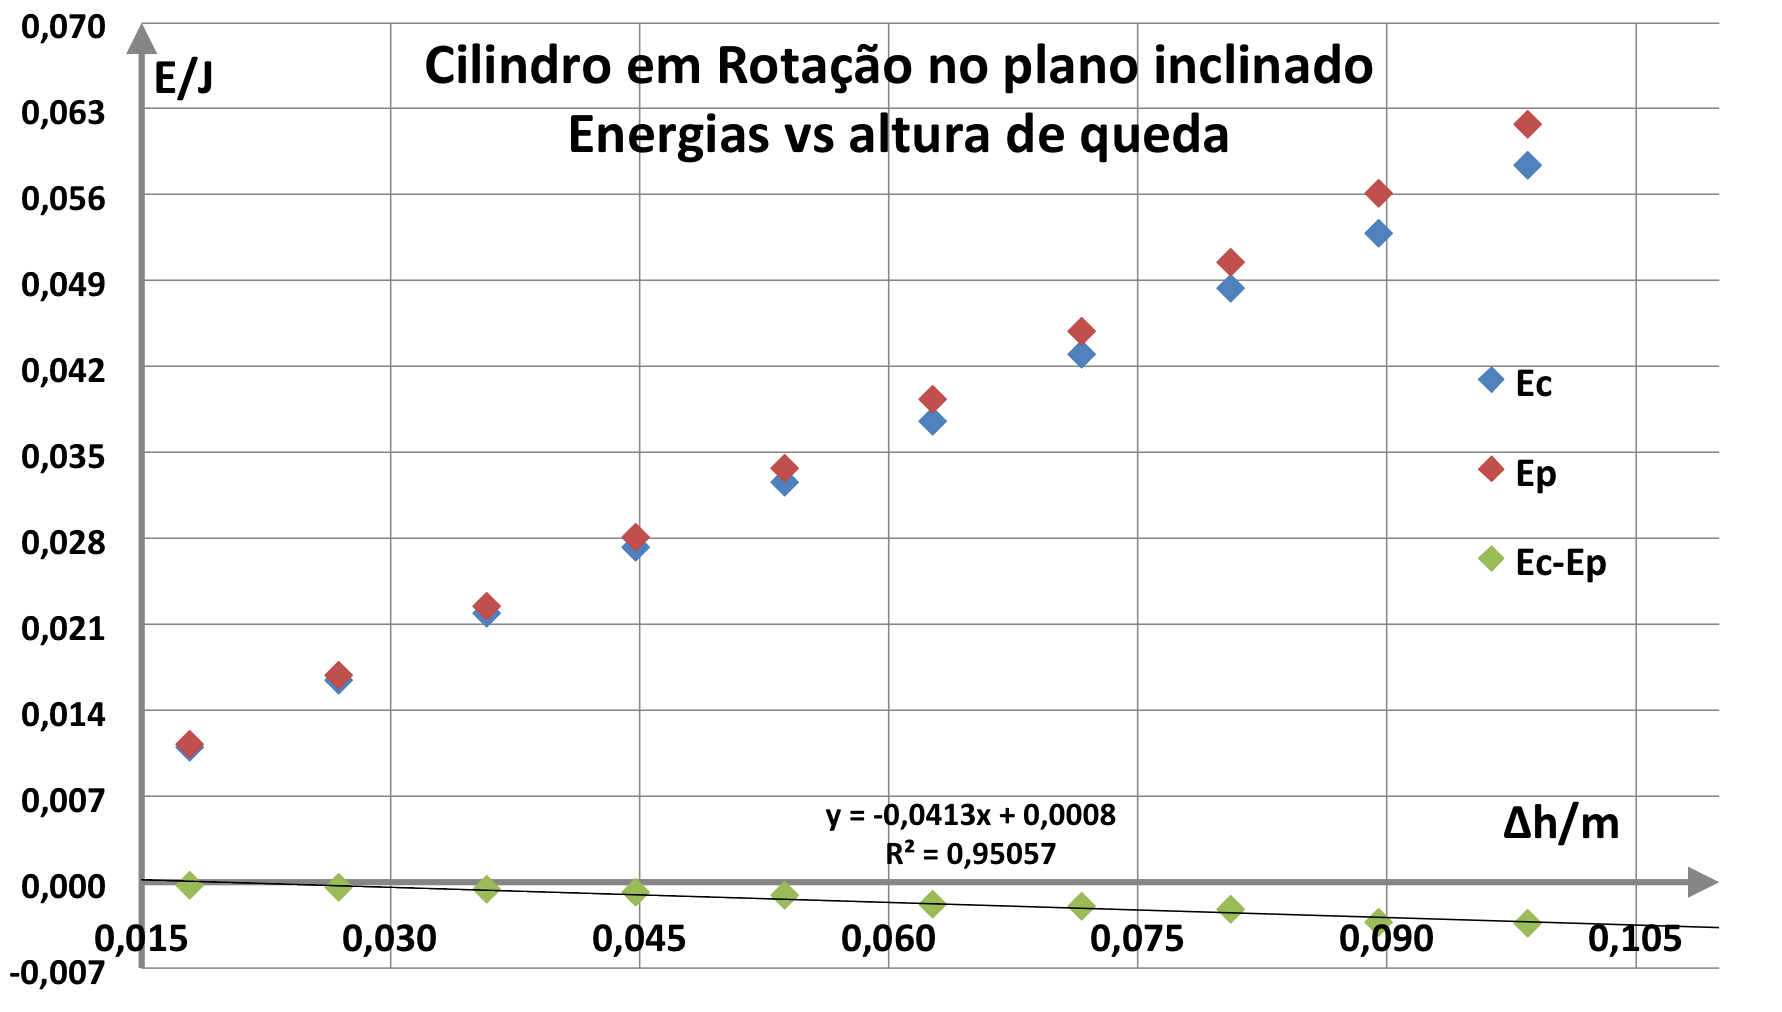
\includegraphics[width=120mm]{cilindroPlanoInclinadOrig.png}
%%% legenda da figura
\caption{Cilindro com Rota??o no plano inclinado: energias cin?tica final (Ec), potencial inicial (Ep) e a sua diferen?a (Ec-Ep) em Joules, em fun??o da altura relativa de queda $\Delta h$(m). Par?metros originais.}
\label{fig:cilindroOri}%%% etiqueta identificadora desta figura
\end{figure}

%%%%%%%%%%%%%%%%%%%%%%%%%%%%%%%%%%%%%%%%%%%%%%%%%%%%%%%%%%%%%%%%%%%%%
%%%%%%%%%%%%%%%%%%%%%%%%%%%%%%%%%%%%%%%%%%%%%%%%%%%%%%%%%%%%%%%%%%%%%
\section{An?lise de Resultados}

\notasExplicativasAnaliseResultados %% remover

%%%%%%%%%%%%%%%%%%%%%%%%%%%%%%%%%%%%%%%%%%%%%%%%%%%%%%%%%%%%%%%%%%%%%
\subsection{Resultados do Oscilador Harm?nico Amortecido}

Aos dados obtidos ajustou-se uma equa??o que descreve a desacelera??o for?ada do disco de Pohl (com corrente el?trica $i=0,40$ A, no eletro?man). A fun??o da velocidade $v(t)$ ? do tipo:  
\fequ[eq:ajusteVelPohl]{v(t) = (v_{0}.e^{\lambda t} + a_f.t)\sin(W.t)}
Repare-se que a 1$^a$ velocidade m?xima que se mede, $v_{m1}$, ocorre na $1^a$ oscila??o correspondente a t=T/4 (veja-se a \referir[,]{fig:posVelDiscoPohl}).
A fun??o exponencial observada na \referir{fig:ajusteVel400mAPohl} tem par?metros muito pr?ximos dos obtidos com
o programa \textit{DataStudio} (par?metros A, B, C, cujos valores est?o apresentados na \referir[,]{fig:velPohldatastudio}). A vantagem ? que neste ajuste o valor do par?metro $a_f$ foi mantido constante, pois ? $\approx$ o mesmo para todos os lan?amentos. 
Isto permite que os dados experimentais sejam usados na determina??o de valores mais robustos para $v_0$ e $\lambda$: note-se que a incerteza $\Delta_p$ nos par?metros ajustados varia com $\Delta_p\sim\frac{\sigma}{\sqrt{N-N_p}}$, onde $\sigma$ ? o desvio padr?o dos res?duos no ajuste, $N$ ? a quantidade de dados usados e $N_p$ a quantidade de par?metros a determinar. Neste caso, o ajuste feito com \textit{Mathematica} d?:
\begin{itemize}%%% lista de itens, iniciados por s?mbolos escolhidos.
\itemsep -0.1mm
%% O s?mbolo que inicia cada item ? dado entre [ ] 
\item[A=] $v_{0}=+0,9687$ m/s, que ? o par?metro da velocidade. Note-se que ? superior ao primeiro valor medido (no instante $t=T/4$), porque o sistema perde energia continuamente.

\item[B=] $a_f=-0,0027\rm\, m/s^2$, que representa a acelera??o da fric??o mec?nica na rota??o. Foi previamente determinado com os dados de todos os lan?amentos feitos.

\item[C=] $\lambda=-0,2140\,\rm s^{-1}=\frac{1}{T_f}$, onde $T_f=4,673$ s, ?  a constante de tempo da fric??o electromagn?tica.
\end{itemize}

\begin{figure}[h!]%%%  h=here => coloque a figura 'aqui' no texto
\centering
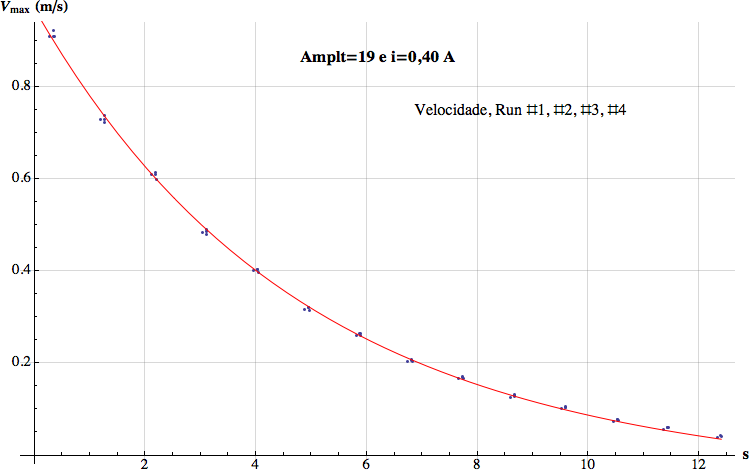
\includegraphics[width=110mm]{HMSajuste_A19i400mA.png}
%%% legenda da figura
\caption{Velocidade linear m?xima (m/s) de rota??o do disco de Pohl, e ajuste da equa??o \ref{eq:ajusteVelPohl}.}
\label{fig:ajusteVel400mAPohl}%%% etiqueta identificadora desta figura
\end{figure}

Este modelo funciona bem mesmo para atenua??es fracas, situa??o em que o modelo de ajuste no \textit{DataStudio} (ou \textit{Excel}) n?o funciona. Veja-se o caso duma corrente el?trica $i=0,05$ A, na \referir{fig:ajusteVel50mAPohl}. Daqui deduzem-se os seguintes par?metros:

% inclus?o de uma figura presa nesta posi??o do texto. 
\figura[fig:ajusteVel50mAPohl]{100mm}{HMSajuste_A19i50mA.png}
{Velocidade linear m?xima do disco de Pohl com amortecimento fraco, e ajuste da equa??o \ref{eq:ajusteVelPohl}}%% fim da legenda da figura
\begin{itemize}%% lista de itens sem s?mbolos de in?cio.
\itemsep -0.1mm
%% Neste texto n?o h? s?mbolo a iniciar cada item pois usa-se [] <-- vazio
\item[] $v_{0}=+1,0071$ m/s, ? o par?metro da velocidade.
\item[] $a_f=-0,0027\rm\, m/s^2$, acelera??o da fric??o mec?nica na rota??o, previamente determinada.
\item[] $\lambda=-0,0231\,\rm s^{-1}\Rightarrow T_f=43,3$ s = constante de tempo da fric??o electromagn?tica.
\end{itemize}


? evidente que uma atenua??o $\approx 10\times$ menor permite um coeficiente $\lambda$ menor (neste fator), e um tempo de amortecimento $X$ vezes maior, quando comparado com a primeira situa??o. O valor de $X$ ? determinado igualando a velocidade m?xima nos dois casos. 
Escolhendo 0,03 m/s,
%% para apresentar equa??es numeradas, num par?grafo separado, use:
\begin{equation}
v1_{0}.e^{\lambda_1 t_1} + a_{f}.t_1 = v2_{0}.e^{\lambda_2 t_2} + a_{f}.t_2 = 0,03
\end{equation}
\noindent
deduz-se que $X=t1/t2=12,68/67,44=5,32$ , como se pode estimar pelos gr?ficos.


%%%%%%%%%%%%%%%%%%%%%%%%%%%%%%%%%%%%%%%%%%%%%%%%%%%%%%%%%%%%%%%%%%%%%
\subsection{Resultados da acelera??o \textit{g} e conserva??o de energia no p?ndulo}

%%% Se n?o quiser usar este \FIGcomTextoaolado comente as linhas respectivas:
\FIGcomTextoaolado[fig:Tpendulo]{4}{90mm}{periodoPenduloGrande2014.png}
{Histograma com a distribui??o dos per?odos medidos. Note-se a distribui??o gaussiana que se aproxima bastante bem ao histograma dos dados.}%%<<-- LEGENDA
%%% O texto seguinte deve estar sem linha de separa??o (vazia).
O histograma das 1038 medi??es do per?odo do p?ndulo grande no lab.\ C1.4.31 est? apresentado na \referir{fig:Tpendulo}. O valor m?dio deste per?odo leva a deduzir que: 
%%% etiqueta da equa??o: eq:g
\fequ[eq:g]{g=4\pi^2\frac{l}{T^2}=9,8031\pm 0,0003\,\rm m/s^2}
onde $l=3,3543\pm0,0003 \rm\,m$ (\textit{\small que foi medido com muito sacrif?cio!}) e $T\!=3,6753\pm0,0003\rm\,s$. Dos 1038 dados iniciais, 10 valores foram rejeitados por estarem desviados da m?dia mais de $3,33\,\sigma$ e, estatisticamente, nenhum caso destes deveria ter ocorrido \cite{fisexp}. A incerteza relativa de $g$ demonstra a ?ptima qualidade do resultado: \quad (da \referir[]{eq:g})
$$\Delta g_{rel}=0,017\,\%$$ 

%% Para ter a fig anterior separada do texto, descomente as linhas respectivas.
%% [h!]=here => coloca a fig 'aqui'.  Pode ser combina??es de:
%% [t] (top) ou [b] (bottom) da p?gina, <=> ?s prefer?ncias: [htb]\
%%
%\begin{figure}[h!]
%\centering
%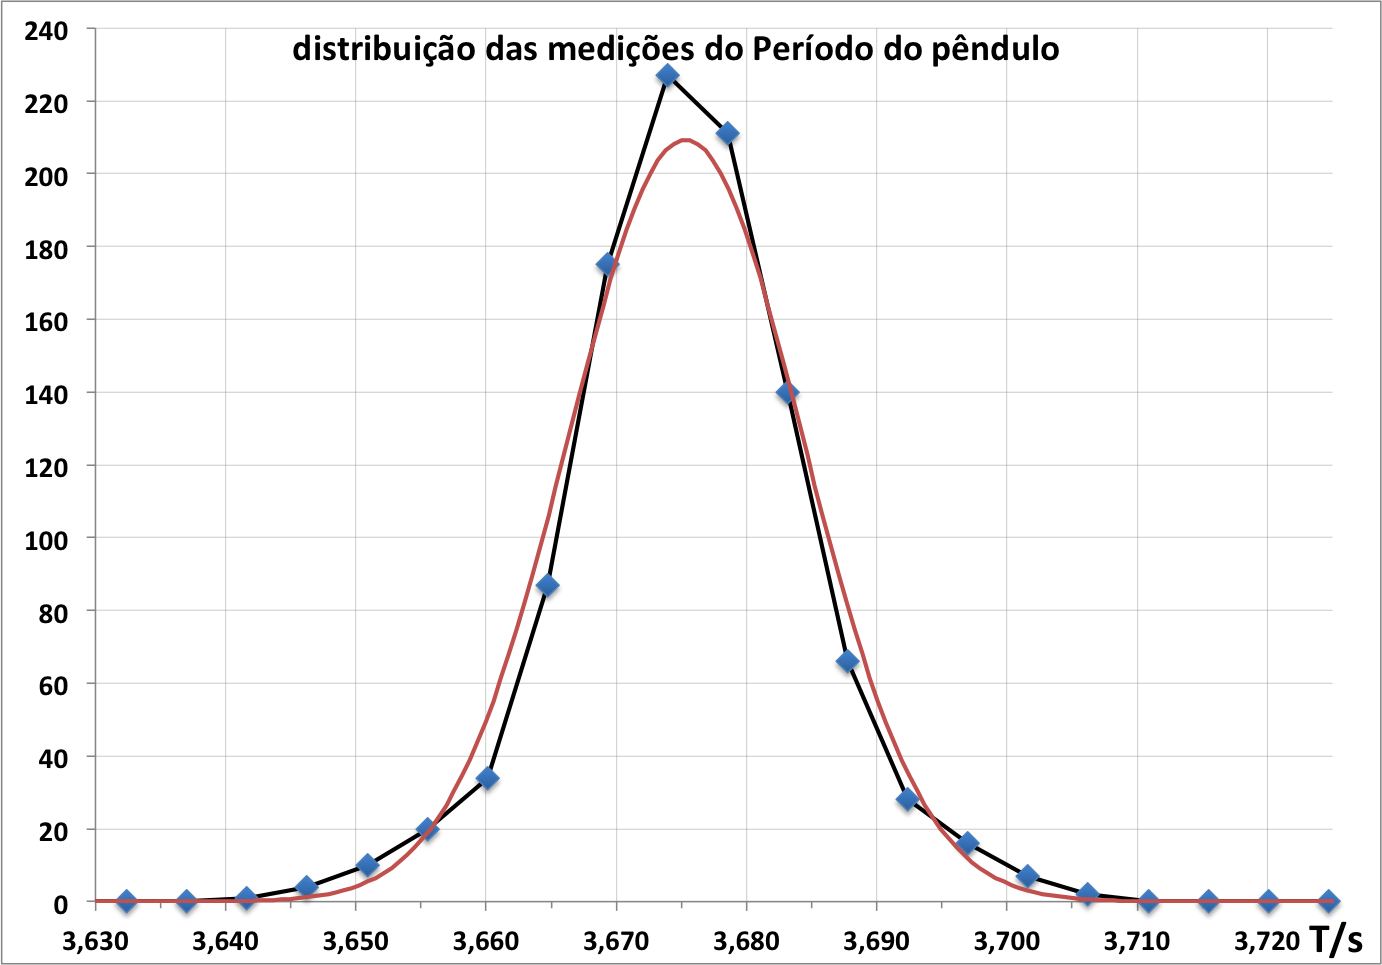
\includegraphics[width=100mm]{periodoPenduloGrande2014.png}
%\caption{Histograma com a distribui??o dos 1038 per?odos $P$ medidos. Note-se a distribui??o gaussiana que se aproxima bastante bem ao histograma dos dados.}%%legenda
%\label{fig:Tpendulo}%%% etiqueta identificadora desta figura
%\end{figure}

\vspace*{-1.8mm}
\FIGcomTextoaolado[fig:velocidPendGrande]{2}{88mm}{velocMaxPenduloGrande2014.png}
{Perda de energia cin?tica: velocidade m?xima do p?ndulo grande, e ajuste de uma reta.}%%<<-- LEGENDA
A conserva??o da energia no p?ndulo tamb?m \textit{n?o} se verifica. Na \referir{tab:dados1.1DataStudio} nota-se que apesar do per?odo se manter praticamente constante, em acordo com o resultado para pequenas oscila??es, a velocidade m?xima diminui em cada passagem. Isto corresponde a perda de energia total no movimento, essencialmente por fric??o aerodin?mica: nota-se bem nestes  dados que a perda de velocidade ? mais r?pida em $V_2$, pois inicia o movimento com um valor superior ao de $V_1$. Mesmo no p?ndulo grande com $l=3,5\,m$ e de baixo atrito, essa perda ? bem vis?vel, como se constata na \referir[]{fig:velocidPendGrande}.

\vspace*{0mm}
%%%%%%%%%%%%%%%%%%%%%%%%%%%%%%%%%%%%%%%%%%%%%%%%%%%%%%%%%%%%%%%%%%%%%
\subsection{Resultados da Conserva??o da Energia Mec?nica}

Um dos principais problemas na verifica??o da conserva??o da energia total est? no c?lculo das energias, tanto a cin?tica como a potencial. O valor da energia cin?tica prov?m do valor medido da velocidade, que ? obtida pela raz?o entre o espa?o percorrido pela palheta em frente ao fotoporta. No caso do carrinho n?o existe grande incerteza dada a forma simples da palheta. Os casos da esfera e da cilindro s?o mais problem?ticos pois assume-se que a luz do fotoporta ? cortada pelo di?metro destes objetos (valor que ? usado no \textit{DataStudio} para calcular a velocidade), quando \textit{n?o h? certeza de se ter colocado o fotoporta exatamente nessa altura}. 

O valor da energia potencial depende da diferen?a de alturas entre a posi??o inicial (de lan?amento) e a do fotoporta (final). Estas alturas tanto foram medidas com fita m?trica em rela??o ao tampo da bancada, como atrav?s por trigonometria usando o ?ngulo de inclina??o da calha de ar e a dist?ncia linear (sobre a calha) entre as duas posi??es. A margem para incerteza ? grande!

Para minimizar estes erros, come?a-se pelo par?metro que afecta todas as experi?ncias e com o caso mais simples, o do carrinho, pois a incerteza prov?m, quase s?, da inclina??o $\alpha$ da calha. Escolheu-se um valor de $\alpha$ que minimizasse as diferen?as entre os valores de energia, mas \textit{impondo a condi??o} $E_c\le E_p$, visto haver perdas por atrito. Assim, em vez do valor inicialmente medido $\alpha_m=5,135^{\rm o}$, usou-se $\alpha=5,418215^{\rm o}$, cujo resultado apresenta-se no gr?fico da \referir{fig:carroCorrig}. Esta pequena diferen?a traduz-se num desn?vel (a mais) entre os extremos da calha de 9,8 mm, que poder? ser devido ? n?o horizontalidade das bancadas entre si e dos pr?prios tampos (?), que n?o se medem com o procedimento habitual, ou erros nas medi??es efetuadas. Note-se que mesmo assim, ainda h? uma perda sistem?tica de energia de 0,0016 J, em cada lan?amento do carrinho. Este facto poder? denunciar um enviesamento na medi??o das dist?ncias entre os pontos de lan?amento e da fotoporta\ldots
%%%
%%% Se quiser ver um exemplo da \FIGcomTextoaolado descomente as linhas seguintes...
%\FIGcomTextoaolado[fig:carroCorrig]{4}{90mm}{translacaoPlanoInclinadCorrig.png}
%{Lan?amentos do Carrinho no plano inclinado: energias cin?tica final (Ec), potencial inicial (Ep) e a sua diferen?a (Ec-Ep) em Joules, em fun??o da altura relativa de queda $\Delta h$(m). Par?metros corrigidos.}%% legenda

%% ...e comente todas as linhas desta figura, que estao a seguir.
\begin{figure}[h!]
%%%  h=here => coloque a figura aqui no texto
\centering %% fig centrada na p?gina
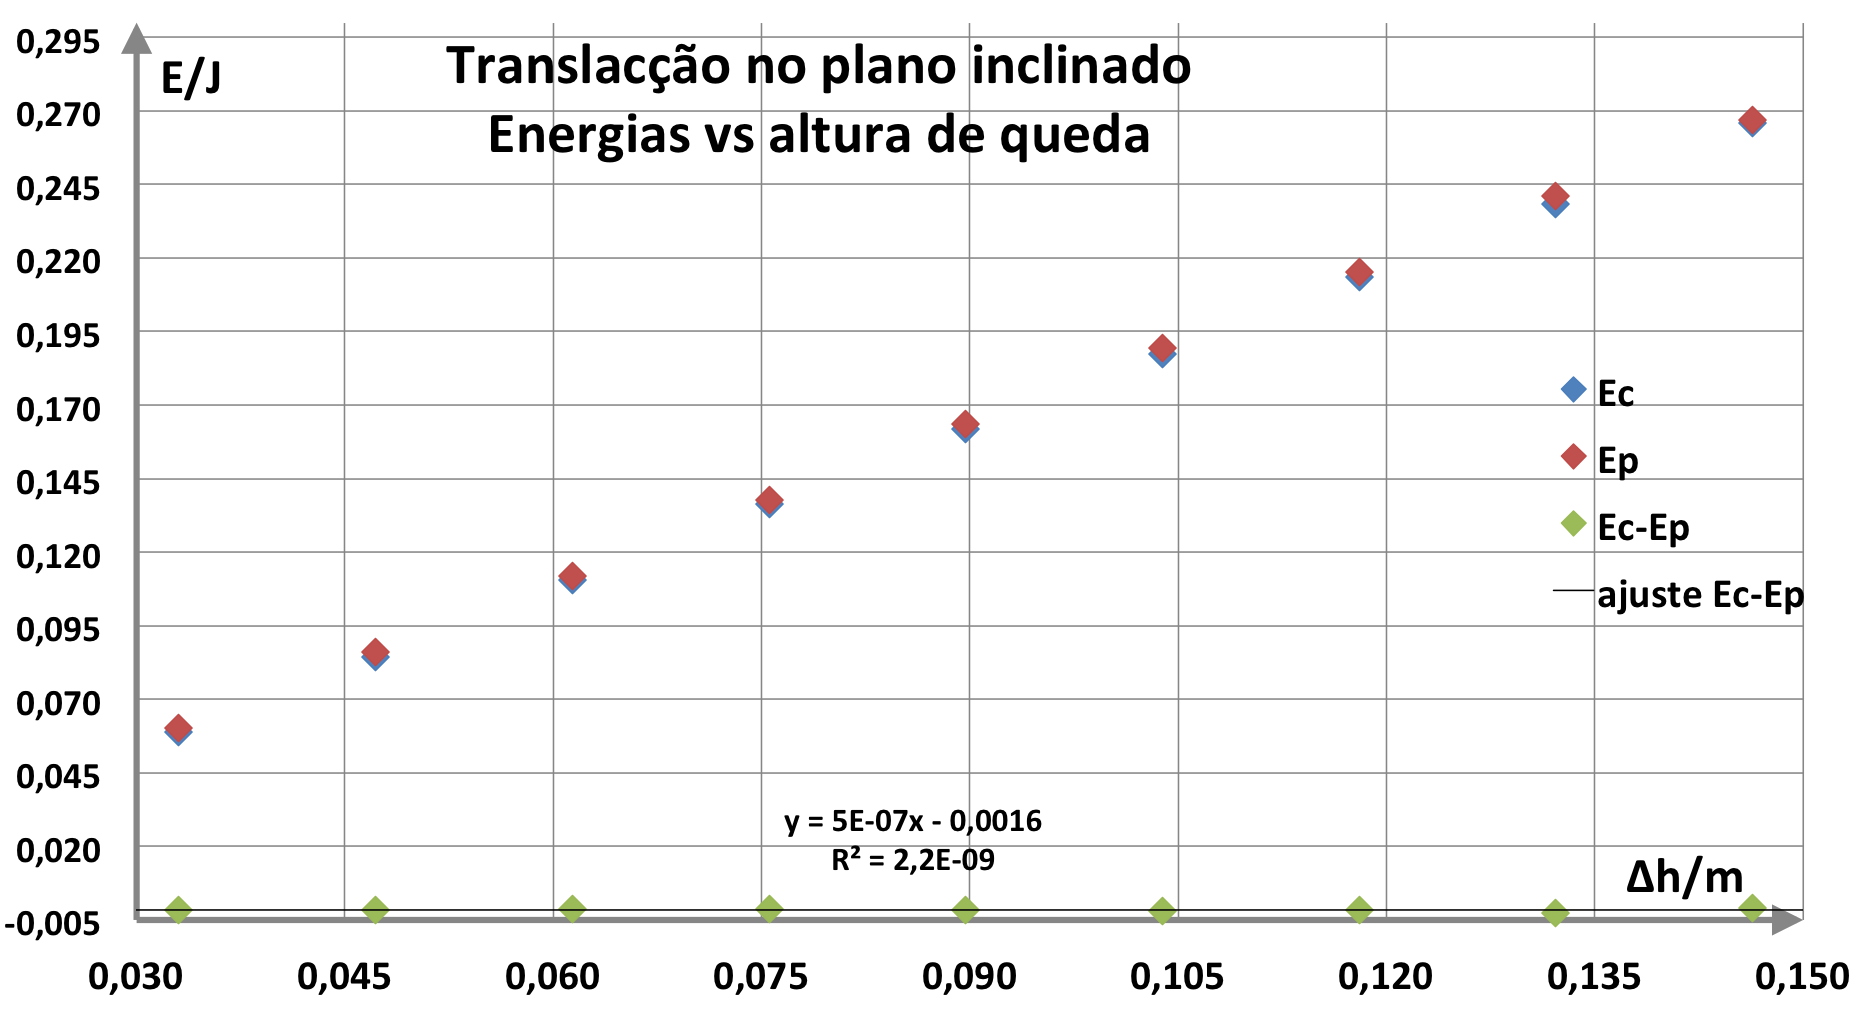
\includegraphics[width=120mm]{translacaoPlanoInclinadCorrig.png}
%%% legenda da figura
\caption{Lan?amentos do Carrinho no plano inclinado: energias cin?tica final (Ec), potencial inicial (Ep) e a sua diferen?a (Ec-Ep) em Joules, em fun??o da altura relativa de queda $\Delta h$(m). Par?metros corrigidos.}
\label{fig:carroCorrig}%%% etiqueta identificadora desta figura
\end{figure}

Nos lan?amentos da esfera e do cilindro foi introduzido o valor de $\alpha$ acima mencionado. Contudo, para encontrar uma solu??o satisfat?ria foi necess?rio considerar que a luz do fotoporta passava numa corda (do objeto) de comprimento $D'$  diferente do seu di?metro $D$, em todas as experi?ncias realizadas. Teoricamente, a velocidade medida na corda $D'$ ? a mesma que a velocidade do objeto $v=D/\Delta t=D'/\Delta t'$. Por?m, o valor de velocidade apresentado pelo \textit{DataStudio}, $v'=D/\Delta t'$, ? diferente de $v$, pelo facto de se lhe ter introduzido o di?metro $D$ em vez de $D'$, \textit{que era desconhecido}.
A rela??o entre as duas ser?:
\[
v'=\frac{D}{\Delta t'}=\frac{D}{D'}\frac{D'}{\Delta t'}=\frac{D}{D'}v
\;\Leftrightarrow\; v= \frac{D'}{D}v'
\]

Para os dados obtidos, encontrou-se o valor $D'$ que minimiza as diferen?as entre os valores de energia, mas \textit{impondo a condi??o} $E_c\le E_p$, visto haver perdas por atrito. Note-se que esta metodologia no tratamento de dados \textbf{n?o ? boa} para quem fez as experi?ncias largando o objeto sempre da mesma posi??o inicial e colocando o fotoporta ao longo da calha. Nessa situa??o, o valor de $D'$ foi diferente para cada posi??o final escolhida, devido ao ajustamento constante na altura do fotoporta.

Para o lan?amento da esfera em rota??o, apresentam-se na figura \ref{fig:esferaCorrig} os resultados tratados com  $D'$=19,12 mm, valor da corda que passou no fotoporta ao inv?s do di?metro $D$=20,0 mm da esfera. ? evidente que a medi??o referente aos 2,8 cm de altura mant?m o desvio desproporcionado ao dos outros dados, mas corrigiu-se o aumento da energia total do sistema: parece haver uma perda sistem?tica de 0,0007 J. O declive positivo est? a ser for?ado pelo valor\footnote{Tudo indica que esta medi??o ficou mal feita e por isso o valor est? muito desviado dos outros.} a $\Delta h=2,8$ cm.
\begin{figure}[h!]
%%%  h=here => coloque a figura aqui no texto
\centering %% fig centrada na p?gina
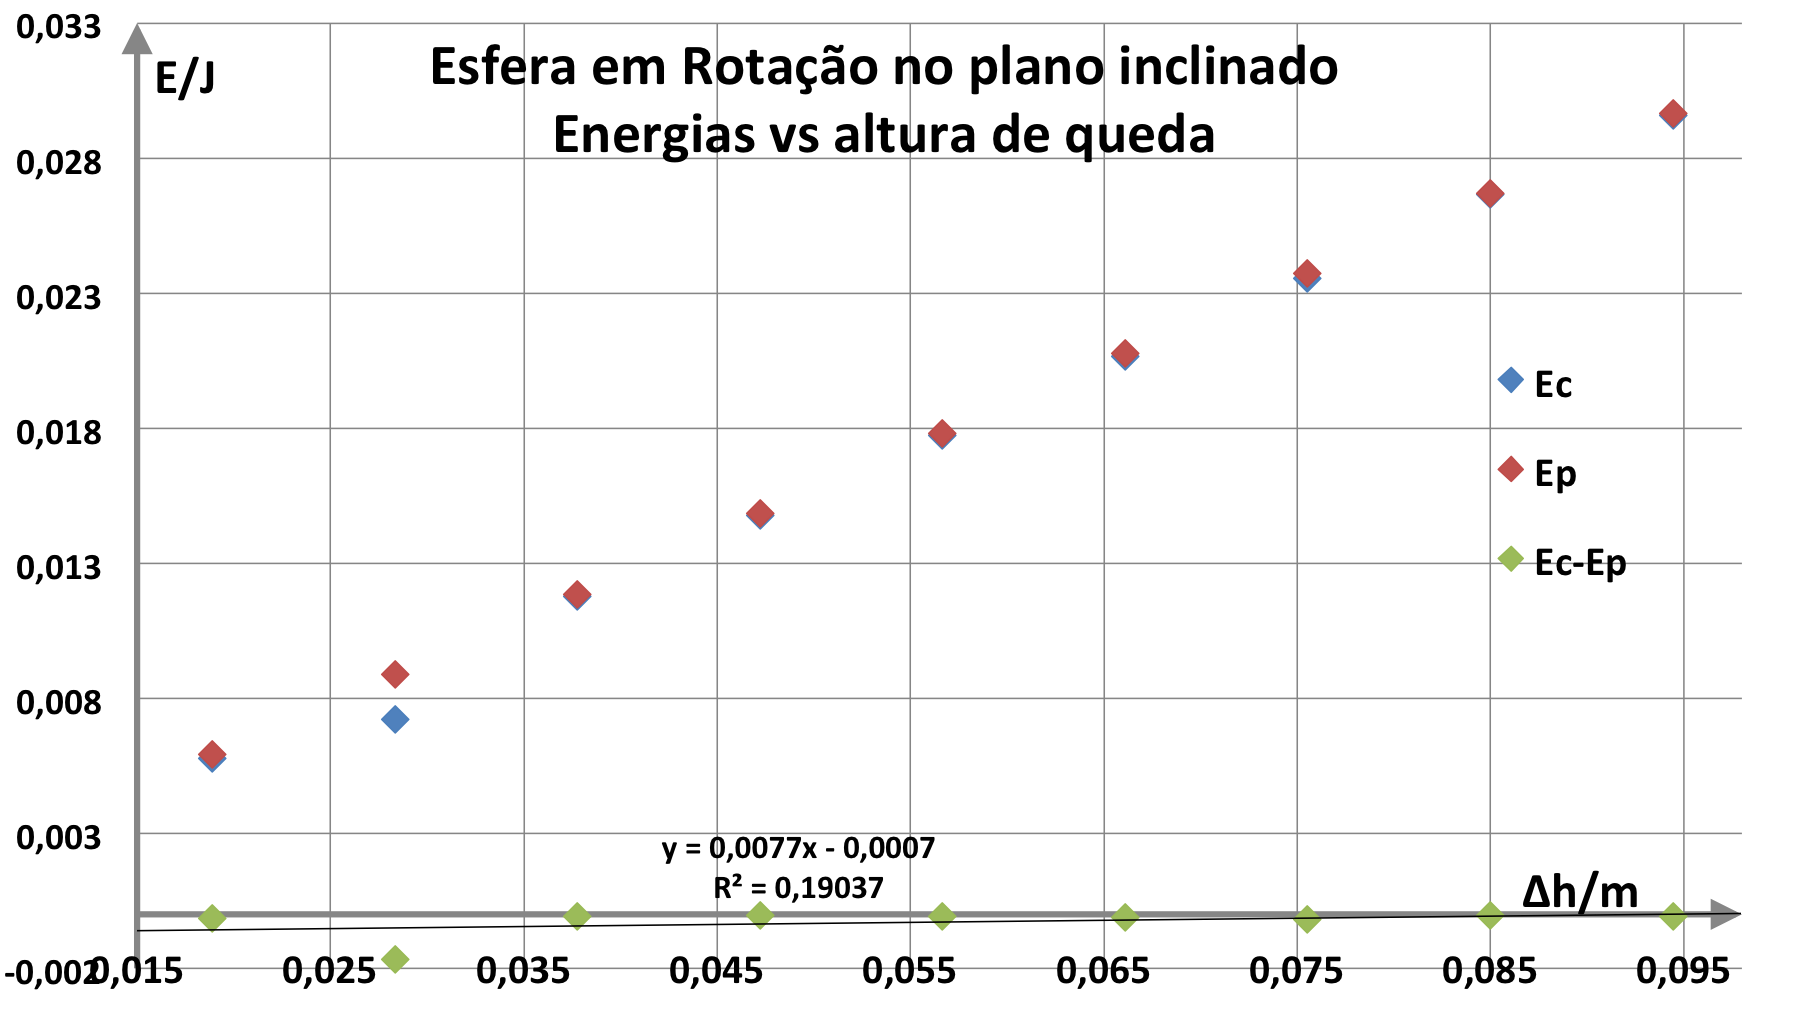
\includegraphics[width=110mm]{esferaPlanoInclinadCorrig.png}
%%% legenda da figura
\caption{Esfera em rota??o no plano inclinado: energias cin?tica final (Ec), potencial inicial (Ep) e a sua diferen?a (Ec-Ep) em Joules, em fun??o da altura relativa de queda $\Delta h$(m). Par?metros corrigidos.}
\label{fig:esferaCorrig}%%% etiqueta identificadora desta figura
\end{figure}

Com os dados do lan?amento do cilindro a diversas alturas iniciais procedeu-se da mesma maneira, introduzindo-se $D'$=20,40 mm, como valor da corda que passou no fotoporta (deve incluir o pequeno anel de guiagem) ao inv?s do di?metro que o cilindro tem, $D$=19,64 mm, usado na \referir{fig:cilindroOri}. Os resultados apresentam-se na \referir{fig:cilindroCorrig}: nesta situa??o h? uma perda de energia total mais evidente: a diferen?a $E_c-E_p$ aumenta visivelmente com a altura do lan?amento. 
\begin{figure}[h!]
%%%  h=here => coloque a figura aqui no texto
\centering %% fig centrada na p?gina
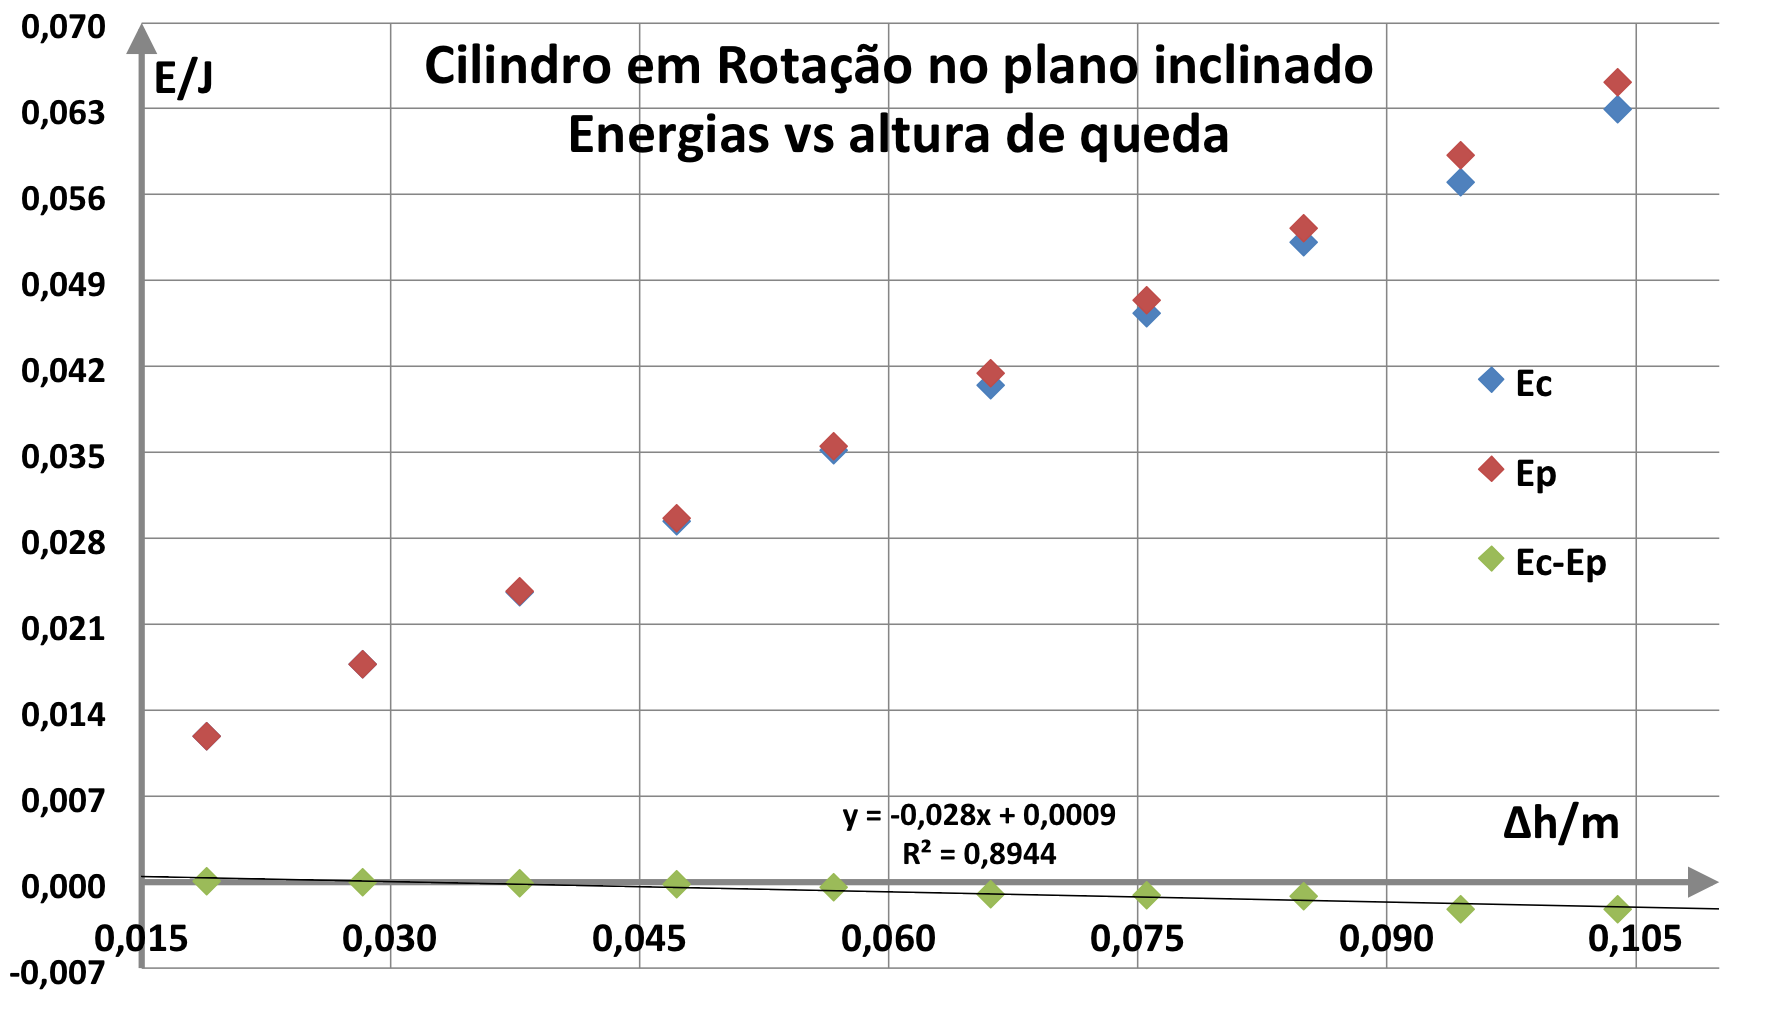
\includegraphics[width=110mm]{cilindroPlanoInclinadCorrig.png}
%%% legenda da figura
\caption{Lan?amentos do Cilindro no plano inclinado: energias cin?tica final (Ec), potencial inicial (Ep) e a sua diferen?a (Ec-Ep) em Joules, em fun??o da altura relativa de queda $\Delta h$(m). Par?metros corrigidos.}
\label{fig:cilindroCorrig}%%% etiqueta identificadora desta figura
\end{figure}


%%%%%%%%%%%%%%%%%%%%%%%%%%%%%%%%%%%%%%%%%%%%%%%%%%%%%%%%%%%%%%%%%%%%%
%%%%%%%%%%%%%%%%%%%%%%%%%%%%%%%%%%%%%%%%%%%%%%%%%%%%%%%%%%%%%%%%%%%%%
\section{Discuss?o dos Resultados e Conclus?es}
%%%%%%%%%%%%%%%%%%%%%%%%%%%%%%%%%%%%%%%%%%%%%%%%%%%%%%%%%%%%%%%%%%%%%

\notasExplicativasResultadosConclusoes%% a eliminar

\begin{enumerate}%% lista numerada
\itemsep -0.mm
\item
Como o valor correcto\footnote{medi??es gravim?tricas do Prof. Carlos Antunes, do DEGGE} 
da acelera??o grav?tica para o 4$^o$ piso do C1 ? $g=9,8007\rm\, m/s^2$, o resultado obtido na equa??o \vref{eq:g} tem um erro absoluto 
\fequ{\Delta g_{abs}=9,8031-9,8007 = +0,0024\pm 0,0003 \rm\, m/s^2} 
que se deve ? conjun??o de Marte com Neptuno na semana em que a experi?ncia decorreu. \textit{Ficou indubitavelmente provado} que a pequena atra??o destes dois planetas aumentou um pouco o valor de $g$ no edif?cio C1.

\item
As medi??es com a calha de ar inclinada permitiram demonstrar a conserva??o da energia total (mec?nica) no caso do carrinho, sendo necess?rio contudo, reajustar os par?metros experimentais que n?o foram (ou n?o podiam ser) medidos com grande rigor.

Nos objetos com rota??o, mostrou-se que h? maior perda de energia no caso do cilindro, apesar da massa ser o dobro da da esfera. A nossa interpreta??o ? que durante a descida, os movimentos de oscila??o lateral faziam o anel de guiagem ir batendo no sulco, al?m da superf?cie de contacto com a r?gua ser maior. Por isso, as for?as de atrito foram mais intensas e, proporcionais ao espa?o percorrido (altura de largada), ou seja, o trabalho destas for?as ? realizado num percurso maior. No caso da esfera, o atrito limitou-se ao encosto da sua superf?cie nas quinas do sulco de guiagem na r?gua, que deve ser diminuto como os resultados demonstram (fig.\  \vref{fig:esferaCorrig}).

\item
A an?lise estat?stica dos resultados obtidos na \referir{tab:dados} prova que o universo est? em \textit{contra??o acelerada} e que o \textbf{colapso total} ocorrer? no pr?ximo m?s de Junho, antes dos exames finais na FCUL. 
Este resultado coloca em quest?o a cren?a generalizada na expans?o acelerada do universo. Contudo o pequeno grau de incerteza nestes resultados leva a \textit{duvidar da pr?pria exist?ncia do universo observ?vel}, o que me impede de assistir ?s aulas nos pr?ximos 3 anos $\clubsuit$.

\item Refor?a-se a ideia de que os resultados obtidos s?o t?o excecionais que ser?o apresentados na pr?xima confer?ncia planet?ria sobre Astrof?sica trans-observacional.

\end{enumerate}


%%%%%%%%%%%%%%%%%%%%%%%%%%%%%%%%%%%%%%%%%%%%%%%%%%%%%%%%%%%%%%%%%%%%%
%%%%%%%%%%%%%%%%%%%%%%%%%%%%%%%%%%%%%%%%%%%%%%%%%%%%%%%%%%%%%%%%%%%%%
%%%% Se n?o tiver refer?ncias a incluir "comente" TODAS as linhas 
%%%% seguintes, ou seja, inicie-as por % ou apague-as.
%%%%%%%%%%%%%%%%%%%%%%%%%%%%%%%%%%%%%%%%%%%%%%%%%%%%%%%%%%%%%%%%%%%%%
\begin{referencias}
%% Cada livro, artigo, etc., que foi usado neste estudo, deve indicar-se como
%% nas refer?ncias. Para isso usa-se o c?digo '\bibitem{label} nome..' 
%%  onde label=codigo da ref que ? usada no texto: \ref{label}
%%
%% Se quiser disponibilizar os seus dados num site p?blico inclua aqui 
%%  a refer?ncia, que deve existir mesmo!!
\bibitem{nossosdados} \listaAutores,%%<<---esta vari?vel predefinida
%% cont?m a lista de nomes dos autores, separados com v?rgulas.
\emph{Dados da Experi?ncia da Conserva??o da Energia Mec?nica}, no site de acesso p?blico \http{alunos.fc.ul.pt/f1234}. %%% este endere?o ? fict?cio!
Ou envie-nos um e-mail para \href{mailto:marta.joaquina@fc.ul.pt}{joaquina.maria@gmail.com}.

\bibitem{fisexp} Concei??o Abreu, Lu?s Matias, Lu?s Peralta, 
\emph{F?sica Experimental, uma Introdu??o}, Ed. Presen?a, 1994.

\bibitem{pendulo} \emph{Pendulum Motion} no site HyperPhysics do Department of Physics and Astronomy, Georgia State University, USA. 
\http{hyperphysics.phy-astr.gsu.edu/hbase/pend.html}.

\end{referencias}

%%%%%%%%%%%%%%%%%%%%%%%%%%%%%%%%%%%%%%%%%%%%%%%%%%%%%%%%%%%%%%%%%%%%%
%%%%%%%%%%%%%%%%%%%%%%%%%%%%%%%%%%%%%%%%%%%%%%%%%%%%%%%%%%%%%%%%%%%%%
\end{document} %%% final do texto do documento